\documentclass[10pt]{article}
\usepackage{icmlko}

\icmlmeta{IP 파운데이션 월드모델}{27}{덜 관측된 학생이었다}{팝업에서 두 축을 빼자 게임보다 어려워졌다 --- 게임의 난이도는 도메인 성질이 아니라 관측 부족이다}

\begin{document}

\twocolumn[
\icmlheader

\begin{abstract}
노트 24는 게임을 ``매우 나쁜 학생''으로 규정했다. 노트 25가 배선 오류를 고쳐
난이도를 $+$0.0415에서 $+$0.0289로 낮췄지만 여전히 가장 어려운 대상이었고, 남은
부분의 원인은 미결이었다. 이 노트가 반사실로 답한다. \textbf{팝업에서 게임에 없는
두 축(매장 노출도, 입장 허들)을 빼자 팝업이 게임보다 어려워졌다} --- 팝업
$+$0.0238 대 게임 $+$0.0113. 관측 축을 같은 셋으로 맞추면 게임이 오히려 쉬운
대상이다. \textbf{게임의 잔여 난이도는 도메인 성질이 아니라 관측 부족이다.}
노트 24의 ``나쁜 학생'' 규정을 철회한다 --- 게임은 나쁜 학생이 아니라 \emph{덜
관측된} 학생이었다. 함께 노트 26이 남긴 제거 강도 곡선도 그렸다. 팝업 제1주성분을
$\alpha$만큼 빼며 전이를 재니 \textbf{$\alpha$=0.2에서 아주 약간 개선되고
($-$0.0780 $\to$ $-$0.0794) 0.4부터 급락한다}($-$0.0175), 0.6에서 부호가 뒤집힌다
($+$0.0706). 제1주성분의 20\% 정도는 빼도 되는 성분일 수 있으나 나머지 80\%는
신호다. 노트 26의 결론이 유지되면서 경계가 정해졌다.
\end{abstract}
]

\section{제거 강도를 조절해 봤다}

노트 26은 팝업 태그의 제1주성분을 통째로 빼자 팝업이 낀 네 방향이 전부 붕괴하는
것을 보고 ``상관은 편향이 아니라 실체''라고 결론지었다. 같은 노트의 한계 절에
``제거 방식이 제1주성분 잔차화 하나뿐이다. 더 온건한 축소에서는 결과가 다를 수
있다''고 적었다.

$\alpha$를 0에서 1까지 두고 제1주성분의 $\alpha$배만 뺐다.

\begin{figure}[t]
\centering
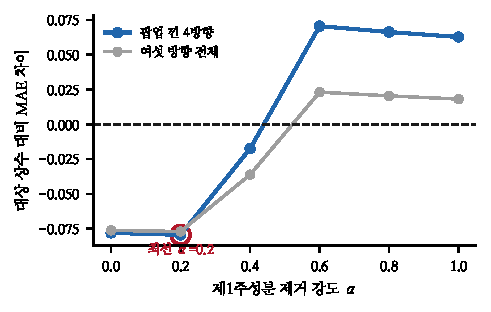
\includegraphics[width=\columnwidth]{figs/shrink.pdf}
\caption{제거 강도와 전이 성능. 0.2까지는 평평하고 0.4부터 급락한다.}
\end{figure}

\begin{table}[t]
\centering\tsize
\caption{제거 강도 곡선. 낮을수록 좋다.}
\begin{tabular}{rrr}
\toprule
$\alpha$ & 팝업 낀 4방향 & 여섯 방향 전체 \\
\midrule
0.0 & $-$0.0780 & $-$0.0762 \\
\textbf{0.2} & \textbf{$-$0.0794} & \textbf{$-$0.0770} \\
0.4 & $-$0.0175 & $-$0.0361 \\
0.6 & $+$0.0706 & $+$0.0232 \\
1.0 & $+$0.0628 & $+$0.0182 \\
\bottomrule
\end{tabular}
\end{table}

$\alpha$=0.2에서 아주 약간 나아진다($-$0.0780에서 $-$0.0794). 개선폭이 0.0014로
미미하므로 실질적 이득이라 하기 어렵다. 중요한 것은 그 뒤의 급락이다 --- 0.4에서
$-$0.0175, 0.6에서 $+$0.0706으로 부호가 뒤집힌다.

\claimx{팝업 제1주성분의 20\% 정도는 빼도 성능이 유지되지만 그 이상 빼면 급격히
무너진다. 노트 26의 결론(상관은 신호다)이 유지되며, 경계가 $\alpha\approx$0.3에
있다.}{다른 도메인의 제1주성분에서도 같은 20\% 경계가 나오면 일반 규칙이고,
도메인마다 다르면 팝업 태깅의 성질이다.}

이 곡선은 노트 26의 진단을 정교하게 만든다. 상관이 전부 실체는 아닐 수 있다 ---
20\%쯤은 후광 편향일 여지가 있다. 그러나 그것을 골라낼 방법이 없고, 넉넉히 빼면
신호를 함께 잃는다.

\section{반사실 --- 팝업에서 두 축을 빼면}

노트 25는 게임의 배선 오류를 고쳐 난이도를 $+$0.0415에서 $+$0.0289로 낮췄지만
게임은 여전히 가장 어려운 대상이었고, ``배선이 원인의 전부는 아니다''를 한계로
남겼다.

남은 원인 후보는 관측 축 수다. 게임은 둘, 아이돌은 넷, 팝업은 다섯을 관측한다.
확인 방법은 반사실이다 --- \textbf{팝업에서 게임에 없는 축을 빼면 팝업이 게임만큼
어려워지는가.}

\begin{figure}[t]
\centering
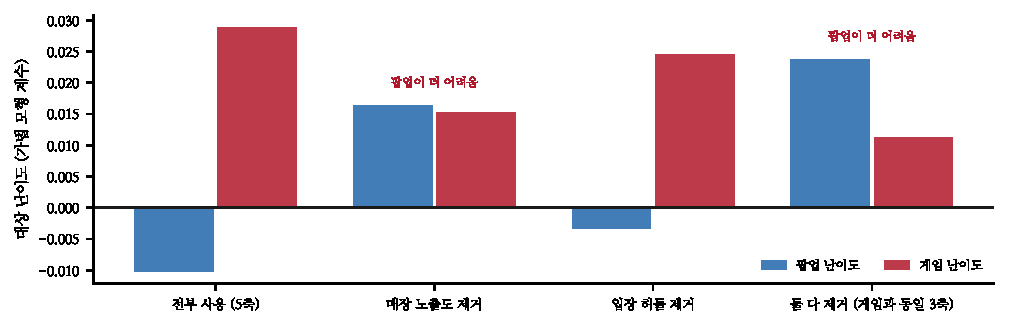
\includegraphics[width=\textwidth]{figs/cf.pdf}
\caption{팝업에서 축을 제거했을 때의 대상 난이도. 둘 다 빼면 팝업이 게임을 넘는다.}
\end{figure}

\begin{table}[t]
\centering\tsize
\caption{반사실 실험. 팝업의 관측 축만 바꾸고 나머지는 그대로 둔다.}
\begin{tabular}{lrr}
\toprule
팝업 구성 & 팝업 난이도 & 게임 난이도 \\
\midrule
전부 사용 (5축) & $-$0.0102 & $+$0.0289 \\
입장 허들 제거 (4축) & $-$0.0034 & $+$0.0245 \\
매장 노출도 제거 (4축) & $+$0.0164 & $+$0.0152 \\
\textbf{둘 다 제거 (3축)} & \textbf{$+$0.0238} & \textbf{$+$0.0113} \\
\bottomrule
\end{tabular}
\end{table}

축을 뺄수록 팝업이 어려워지고, 둘을 다 빼면 \textbf{팝업이 게임보다 어려워진다}
($+$0.0238 대 $+$0.0113). 게임과 같은 조건으로 맞추면 게임이 오히려 쉬운 대상이다.

\begin{figure}[t]
\centering
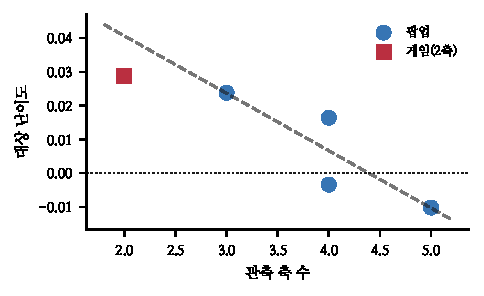
\includegraphics[width=\columnwidth]{figs/ax.pdf}
\caption{관측 축 수와 대상 난이도. 팝업의 네 구성과 게임이 같은 직선 위에 있다.}
\end{figure}

\claimx{게임의 대상 난이도는 도메인 성질이 아니라 관측 축 부족이다. 팝업의 관측
축을 게임과 같은 셋으로 줄이면 팝업이 게임보다 어려워진다.}{축 수를 맞춘 뒤에도
게임이 더 어려운 구성이 나오면 관측 부족만으로는 설명되지 않는다.}

\section{노트 24를 철회한다}

노트 24는 이렇게 썼다.

\begin{quote}\fontsize{9.2}{11}\selectfont
게임은 평범한 선생이고 매우 나쁜 학생이다. \dots\ 게임의 대상 점수 $+$0.0415는
다른 둘($-$0.0172, $-$0.0242)과 자릿수가 다르다.
\end{quote}

두 노트가 그 진단을 무너뜨렸다.

\begin{itemize}[leftmargin=1.1em,itemsep=0.15em]
\item 노트 25 --- 배선 오류를 고치자 $+$0.0415에서 $+$0.0289로 내려갔다.
      ``도메인 성질''의 30\%가 실은 내 배선 실수였다.
\item 이 노트 --- 나머지는 관측 축 부족이다. 조건을 맞추면 게임이 더 쉽다.
\end{itemize}

\textbf{게임은 나쁜 학생이 아니라 덜 관측된 학생이었다.} 그리고 그 관측 부족은
도메인의 숙명이 아니라 우리가 아직 측정 경로를 못 찾은 상태다.

\claimx{노트 24의 ``게임은 매우 나쁜 학생''을 철회한다. 대상 난이도는 도메인의
고유 성질이 아니라 그 도메인에서 관측된 축 수의 함수다.}{관측 축 수가 같은 두
도메인에서 난이도가 크게 다르면, 축 수 말고 다른 도메인 성질이 있다.}

\section{그러면 무엇이 도메인 성질인가}

스물일곱 편에서 ``도메인 성질''로 지목했던 것들이 차례로 다른 것으로 밝혀졌다.

\begin{table}[t]
\centering\tsize
\caption{도메인 성질로 오인했던 것들.}
\begin{tabular}{lll}
\toprule
노트 & 진단했던 것 & 실제 \\
\midrule
13 & 게임은 좋은 선생 & 상대가 쉬운 대상이었을 뿐 (노트 24) \\
15 & 게임 라벨의 시간 구조 & 축 배선 누출 (노트 25) \\
24 & 게임은 나쁜 학생 & 관측 축 부족 (이 노트) \\
26 & 팝업 태그의 후광 편향 & 실제 규모 공변 (노트 26) \\
\bottomrule
\end{tabular}
\end{table}

네 번 모두 도메인을 탓했다가 측정 쪽으로 돌아왔다. 패턴이 뚜렷하므로 규칙으로
적어 둔다.

\begin{quote}\fontsize{9.5}{11.5}\selectfont
어떤 도메인이 유독 다르게 보일 때, 먼저 \textbf{무엇을 얼마나 재고 있는가}를
확인한다. 도메인의 성질이라는 결론은 측정 조건을 맞춘 뒤에만 내린다.
\end{quote}

\section{한계}

\begin{itemize}[leftmargin=1.1em,itemsep=0.15em]
\item 반사실은 팝업 하나에서만 했다. 아이돌에서 축을 빼는 실험은 관측 축이 넷뿐이라
      여유가 적다.
\item 축을 뺀 팝업과 원래 게임은 축 개수만 같을 뿐 축의 종류가 다르다.
      완전한 통제가 아니다.
\item $\alpha$=0.2의 개선폭 0.0014는 잡음 범위일 수 있다. 반복 없이 단일 측정이다.
\item 관측 축 수와 난이도의 관계는 네 점(팝업 3~5축, 게임 2축)에서 그렸다.
\end{itemize}

\section{다음}

\begin{enumerate}[leftmargin=1.3em,itemsep=0.15em]
\item 게임에서 매장 노출도·입장 허들의 측정 경로 재탐색 --- 이제 그 값어치가
      정량화됐다(난이도 $+$0.0289 대부분).
\item 아이돌에서도 반사실 --- 축을 빼면 난이도가 오르는지.
\item 평정자 간 자료 --- 노트 26의 20\% 경계가 후광인지 확인.
\item 네 번째 도메인.
\end{enumerate}

\vspace{0.6em}
\hrule height 0.3pt
\vspace{0.5em}
{\footnotesize
\textbf{참고문헌}\\[0.3em]
Pearl, J. (2009). \emph{Causality: Models, Reasoning, and Inference}, 2nd ed.
Cambridge University Press.\\[0.15em]
Thorndike, E. L. (1920). A constant error in psychological ratings.
\emph{Journal of Applied Psychology}, 4(1), 25--29.\\[0.15em]
Meredith, W. (1993). Measurement invariance, factor analysis and factorial
invariance. \emph{Psychometrika}, 58(4), 525--543.\\[0.15em]
Ben-David, S. et al. (2010). A theory of learning from different domains.
\emph{Machine Learning}, 79(1--2), 151--175.
}

\end{document}
